 %------------------第四章---------------------------
    \newpage
	\section{超声波接近传感器软件设计}
    \subsection{超声波接近传感器的检测策略}
      在配置完成TUSS4470驱动芯片后,即可开始产生脉冲信号并通过超声换能器发送脉冲波。与传统的超声波传感器不同,采用该驱动芯片可发送指定次数、指定脉冲数的脉冲波,这就为我们设计丰富的检测策略提供了硬件基础。考虑到钢化玻璃处于复杂的工厂环境,传感器易受到各种电磁信号以及本身回波信号的叠加干扰,因此增加传感器的稳定性就变得至关重要。\par
      
      本设计采用多次发射脉冲波的检测策略,在发送完一次指定脉冲数的脉冲波之后,传感器就进入检测模式,假如检测到了有效回波,检测标志位加一。连续发射a次脉冲,以a次脉冲波的发射作为一次检测周期,每个检测周期后都会更新检测状态。当一个检测周期内有超过b次检测到有效回波时,判断为检测到物体,DETECTED\_STATE=1,LED灯亮;有效脉冲波的次数小于或等于a次时,判断为未检测到物体,DETECTED\_STATE=0,LED灯灭。如图\ref{检测逻辑流程图}为实现检测逻辑的程序流程图,图\ref{检测状态转移图}为检测状态转移图。
       \begin{figure}[!h]
  		\centering
		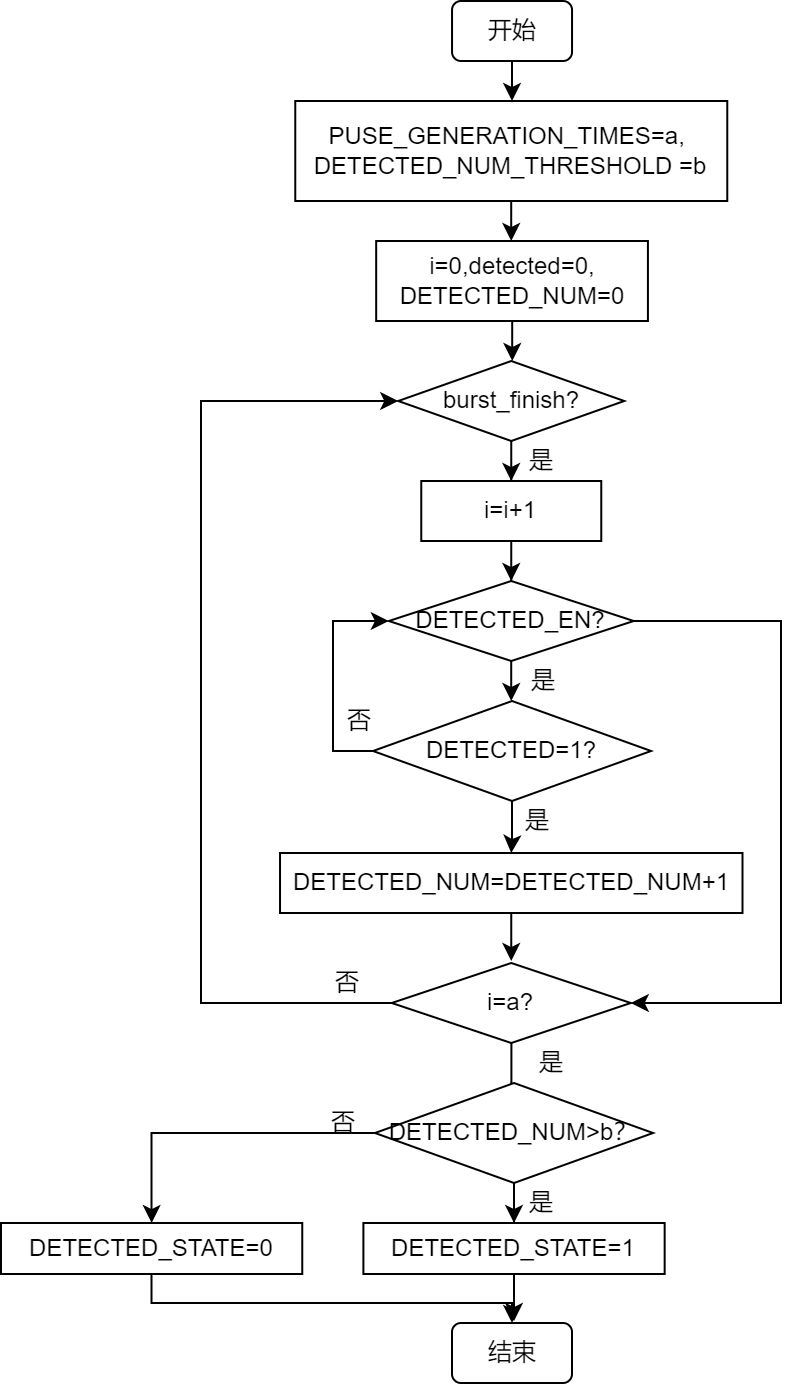
\includegraphics[width=7cm]{figure/detection logic.png}
		\caption{检测逻辑流程图}
		\label{检测逻辑流程图}%文中引用该图片代号
\end{figure}
     \begin{figure}[!h]
	\centering
	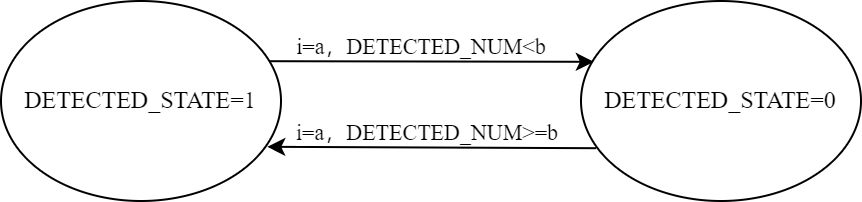
\includegraphics[width=7cm]{figure/LED state transition diagram.png}
	\caption{检测状态转移图}
	\label{检测状态转移图}%文中引用该图片代号
\end{figure}\par
流程图中i用于记录发射脉冲波的次数,PULSE\_GENERATION\_TIMES和DETECTED\_NUM\_THRESHOLD用于定义一个检测周期包括的发射脉冲次数和检测阈值,DETECTED\_NUM用于记录一次检测周期中有效回波的次数,当DETECTED\_NUM超过所设定阈值时,检测状态指示位DETECTED\_STATE就转移为1。\par
    此种检测策略可以极大的增加传感器的稳定性,只有在指定位置持续检测到钢化玻璃时才会认为检测到物体,一定程度上可以避免发生因外界干扰而出现错误检测的情况。
 
     
    \subsection{传感器程序设计}
    \subsubsection{程序总体设计}
    本设计所使用的EPM240T100C5N芯片采用Verilog HDL作为编程语言,Quartus II作为编程烧录软件。Verilog HDL\upcite{Verilog介绍}是一种硬件描述语言(HDL:Hardware Description Language),以文本形式来描述数字系统硬件的结构和行为的语言,用它可以表示逻辑电路图、逻辑表达式,还可以表示数字逻辑系统所完成的逻辑功能。\par
    在本设计中,如图\ref{程序整体框图}所示,将MCU分成四个模块,分别是:MAIN模块、SPI模块、PULSE\_GENERATION模块、DETECTED\_COUNT模块,实现配置TUSS4470芯片、产生脉冲信号、到位指示以及计数等功能。
         \begin{figure}[!h]
        \centering
        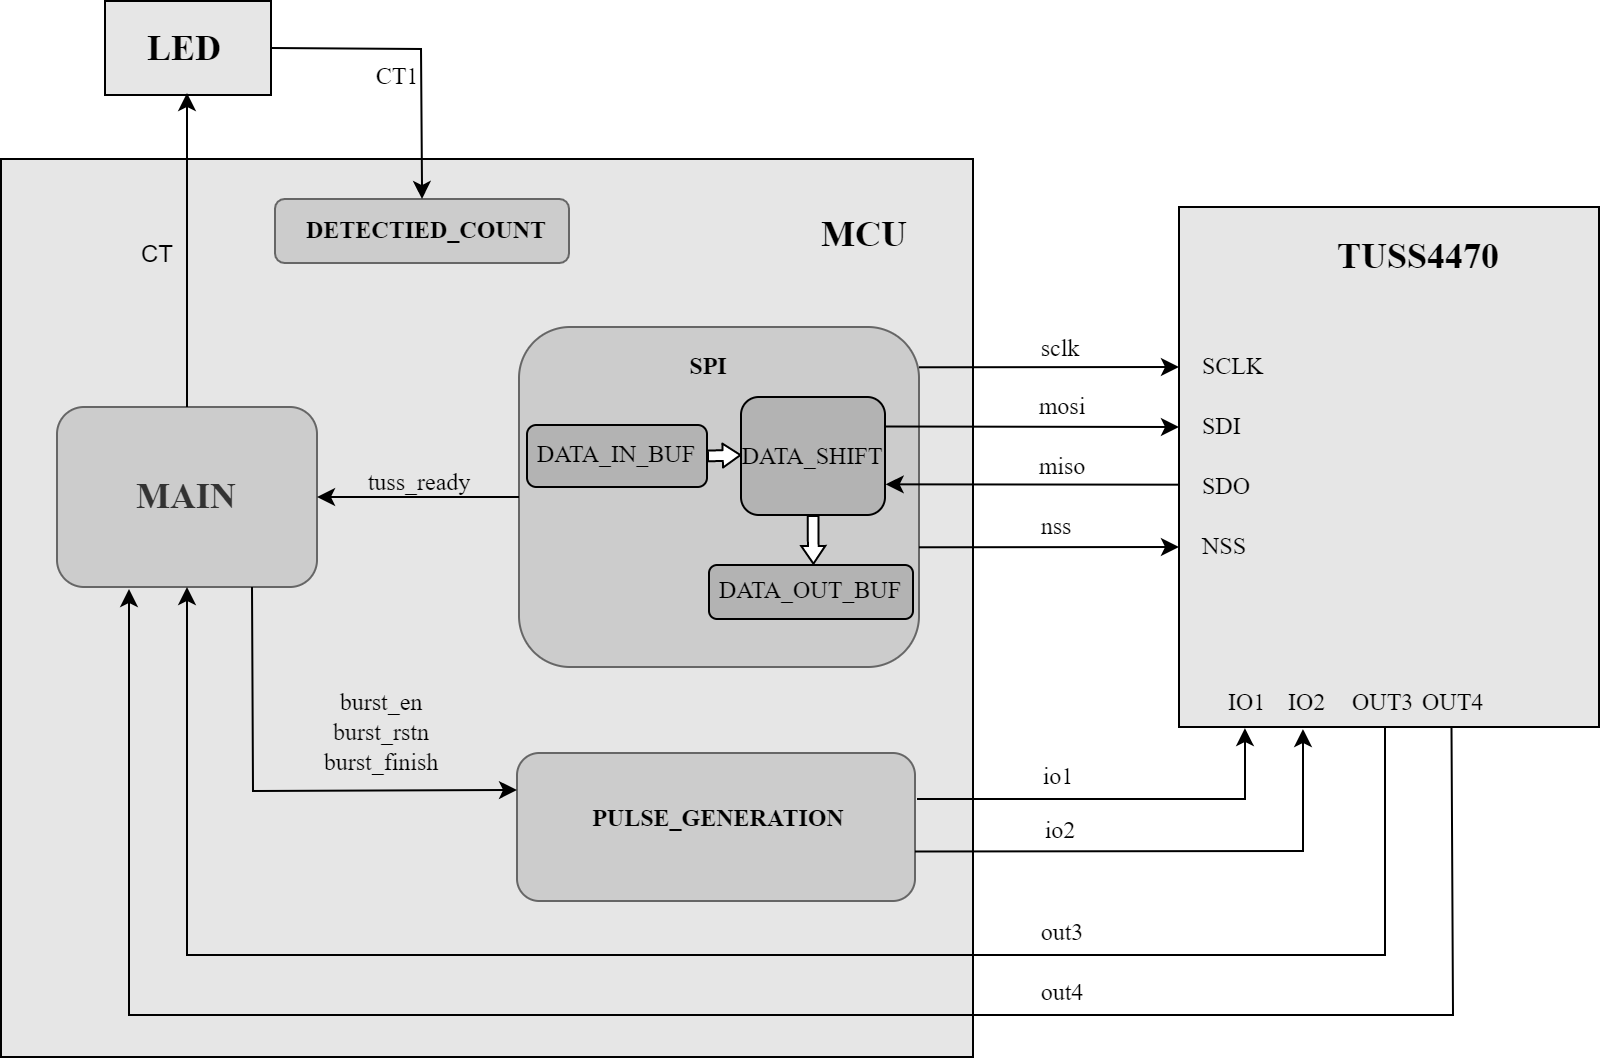
\includegraphics[width=10cm]{figure/Overall program block diagram.png}
        \caption{程序整体框图}
        \label{程序整体框图}
    \end{figure}
    \newpage
    \subsubsection{控制模块}
    
    \paragraph{控制模块功能介绍}
    图\ref{程序整体框图}中的MAIN模块为传感器的控制模块,其作用在于:协调控制各模块的工作,进行主要逻辑判断,是程序的主要部分,图\ref{MAIN模块程序流程图}为MAIN模块的工作流程图。
    首先是SPI模块向TUSS4470芯片发送配置数据,并接收从TUSS4470反馈回的芯片状态;根据反馈数据判断芯片是否准备就绪,当准备就绪后向MAIN模块发送tuss\_ready信号;之后通过IO1、IO2引脚配合控制产生脉冲信号,在每次发送完脉冲信号后,都会根据OUT3、OUT4引脚返回的信息判断本次是否检测到物体;多次检测到预定回波后即确认为检测到物体,通过CT引脚控制LED灯亮;检测计数模块也将进行计数。
    
    \begin{figure}[ht]
        \centering
        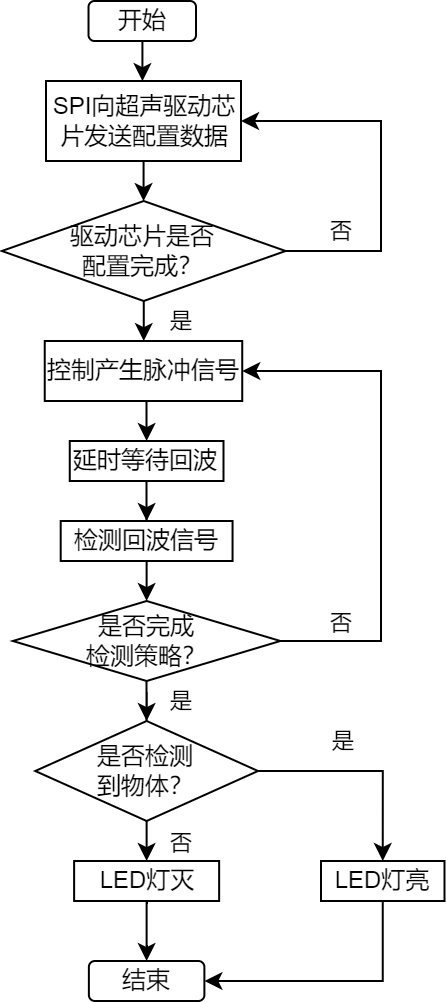
\includegraphics[width=5cm]{figure/MAIN module flow chart.png}
        \caption{MAIN模块程序流程图}
        \label{MAIN模块程序流程图}
    \end{figure}
    
     \noindent
   \paragraph{控制模块逻辑实现}
    MAIN模块的主要逻辑通过状态机的方式来实现,状态机包括了BURST和LISTEN两种状态,对应着超声波传感器发射脉冲信号和接收脉冲信号两种状态。
    
    当TUSS4470芯片配置完成并向MAIN模块发出tuss\_ready信号后,传感器进入到BURST状态,MAIN模块将会向PULSE\_GENERATION模块发送burst\_en信号,使其发射出指定脉冲数的脉冲波,当PULSE\_GENERATION模块完成预期脉冲的发射后,会向MAIN模块发出burst\_finish脉冲发射完成信号,此时MAIN模块将PULSE\_GENERATION模块复位,等待下一次脉冲发射使能。
    
    在每次脉冲发射完成后,都将进入到LISTEN状态,在该状态下,MCU通过检测TUSS4470芯片发出的OUT4信号来判断是否检测到物体,当LISTEN状态保持一段时间后,将会自动跳转到BURST状态,此时就完成了单次的检测,检测次数标志位加一。当完成了一次检测周期的检测时,将根据检测到物体的次数来判断是否进行状态转移,如图\ref{检测状态转移图}所示,在完成状态转移后,检测次数标志位置零,又将进入一次新的检测周期进行检测。
       
    \subsubsection{SPI模块}
	\noindent
    \paragraph{SPI模块介绍}
    在本设计中,MCU芯片通过SPI通信协议来配置TUSS4470芯片。SPI\upcite{SPI}是串行外设接口(Serial Peripheral Interface)的简称,是一种广泛应用于微控制器和数字集成电路之间的通信协议。SPI协议使用四条信号线进行通信,包括时钟信号、数据输入信号、数据输出信号和片选信号。其中时钟信号用于同步数据传输,数据输入和数据输出信号用于传输数据,片选信号用于选择特定的外设设备进行通信。SPI协议的应用范围非常广泛,包括数字信号处理器、微控制器、存储器、传感器、通信模块等。通过SPI协议,这些设备可以快速、可靠地进行数据交换和通信,实现各种复杂的功能和应用。
    
    在本设计中,采用的是四线制SPI,其包括:SCLK(时钟信号)、NCS(片选信号)、MOSI(MCU输出信号)、MISO(MCU输入信号)。SCLK时钟信号和NCS片选信号都由主设备产生,NCS信号拉低为有效信号。
	\noindent
    \paragraph{SPI模块通信模式选择}
    SPI通信模式通过CPOL(时钟极性)和CPHA(时钟相位)来确定。其中CPOL配置SCLK电平的有效态,当CPOL=0时,SCLK低电平处于空闲态,高电平有效,当CPOL=1时,SCLK高电平为空闲态,低电平有效;CPHA配置数据采样发生在第几个边沿,当CPHA=0时,在第一个边沿数据采样,在第二个边沿数据发送,当CPHA=1时,在第一个边沿数据发送,在第二个边沿数据采样。\par
    根据芯片手册可以得知驱动芯片为高电平有效,在上升沿接收数据,在下降沿发送数据,即MCU在上升沿发送数据,在下降沿接收数据,可以得知选择的SPI模式为:CPOL=0,CPHA=1。
    \noindent
    \paragraph{SPI模块实现原理}
    SPI的全双工通信通过一个移位寄存器DATA\_SHIFT来实现。待发送的数据首先写入DATA\_IN\_BUF中进行缓存,需要发送时写入DATA\_SHIFT中,通过移位先将高位数据发送给从机,再将接收到的数据存储到低位,以8位的移位寄存器为例,其工作示意图如图\ref{移位寄存器工作示意图}所示,当发送完成8位数据11110000时,也完成了数据的接收。在接收完成数据后,将数据存入到DATA\_OUT\_BUF寄存器中,至此实现了一帧数据的收发流程。
        \begin{figure}[ht]
        \centering
        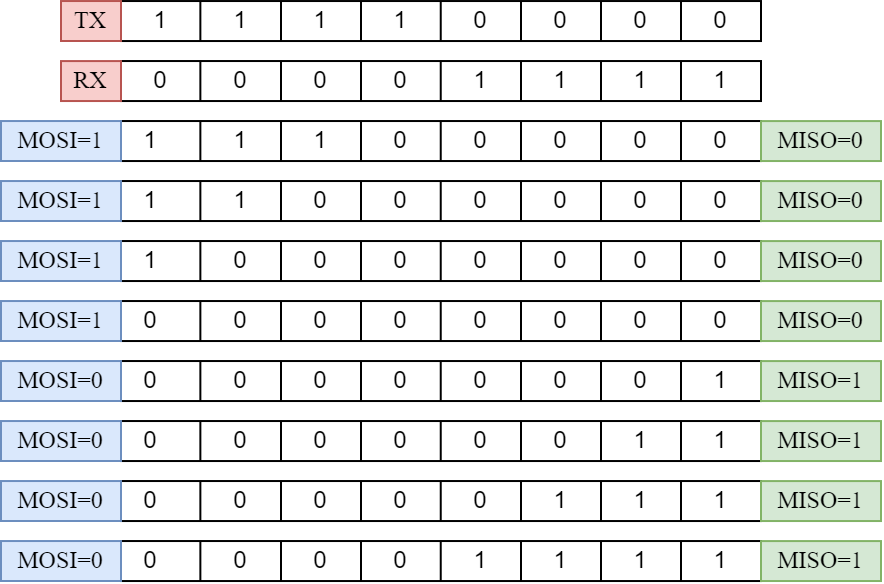
\includegraphics[width=10cm]{figure/DATA_SHIFT.png}
        \caption{移位寄存器工作示意图}
        \label{移位寄存器工作示意图}
    \end{figure}
    \noindent
    \paragraph{SPI模块程序设计}
    线性序列机(linear sequential machine)是一种基于状态转移的有限状态自动机\upcite{线性序列机},常见于数字电路和计算机系统中的控制逻辑设计。线性序列机的基本结构由状态、输入、输出和状态转移四个部分组成。
    
    单帧数据的发送采用线性序列机的方式来实现,即利用一个计数器不断计数,计数器的每一个值都对应一个时刻,在不同时刻对DATA\_SHIFT寄存器采取不同操作,如表\ref{线性序列机}所示。
    \begin{table}[!h]
    	\centering
    	\caption{线性序列机}
    	\begin{GDUTtable}{\textwidth}{Y Y}
    		\textbf{CNT} & \textbf{操作} \\ 
    		\hline
    		复位 & \makecell{DATA\_SHIFT=0;\\DATA\_OUT\_BUF=0; }   \\ 
    		0 & DATA\_SHIFT=DATA\_IN\_BUF;\\
    		1-16 &  \makecell{mosi<=DATA\_SHIFT[15];\\DATA\_SHIFT<={DATA\_SHIFT[14:0],miso};}\\ 
    		17 &    	DATA\_OUT\_BUF<=DATA\_SHIFT; \\ 
    		
    		
    	\end{GDUTtable}
    	
    	\label{线性序列机}
    \end{table}
    
    当复位时,对DATA\_SHIFT寄存器进行初始化;当计数器CNT为0时,将DATA\_IN\_BUF内的数据赋值给DATA\_SHIFT;当CNT为1-16时,DATA\_SHIFT寄存器进行移位操作;当CNT=17时,将DATA\_SHIFT内的数据赋值给DATA\_OUT\_BUF,至此单帧数据收发完毕,在这基础上,将进行多帧数据的收发。
    
    

    
    TUSS4470芯片采用高位先发的方式来收发数据,当NCS信号拉低时,SPI模块开始工作,当NCS拉高,SPI模块停止工作,完成一帧数据的收发。SPI无法实现连续收发多帧的数据,在每帧数据的收发之间NCS需要经历低-高-低的过程。实现多帧数据收发的程序流程图如图\ref{收发多帧数据程序流程图}所示,该程序可一次性发送9帧16位的数据至TUSS4470驱动芯片。
    \begin{figure}[ht]
        \centering
        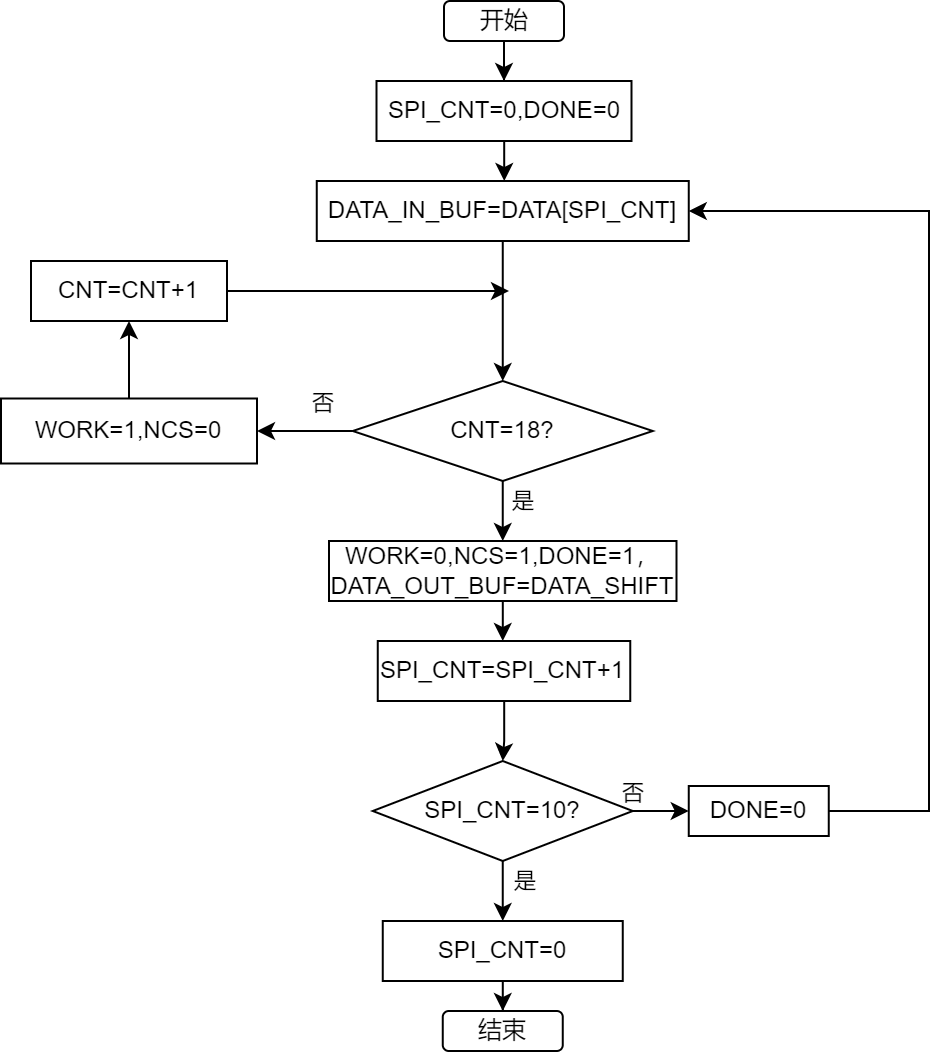
\includegraphics[width=10cm]{figure/SPI Program Flow Chart.png}
        \caption{收发多帧数据程序流程图}
        \label{收发多帧数据程序流程图}
    \end{figure} 
    图中SPI\_CNT用于记录收发数据的帧数;DONE为每帧数据发送完成标志位;WORK为工作位,用于记录工作状态;DATA为一个$10\times16$的数组,用于存放配置数据。
    程序开始运行后,首先进行数据初始化,然后将DATA寄存器内的数据赋给DATA\_IN\_BUF寄存器,片选信号NCS拉低,进行单帧数据的收发。当CNT=18时完成单帧数据的收发,DONE置1,片选信号NCS拉高,帧数计数位SPI\_CNT+1,DONE、CNT置零。在将DATA内的数据发送完成后,根据驱动芯片返回的数据判断芯片是否完成配置,如果完成配置,SPI通信模块将向main模块发送tuss\_ready信号,反之则重新进行配置。
    
    
    

    
    \noindent
    \paragraph{数据结构}
    图\ref{SPI数据结构图1}为SPI通信的数据结构图
    \begin{figure}[ht]
        \centering
        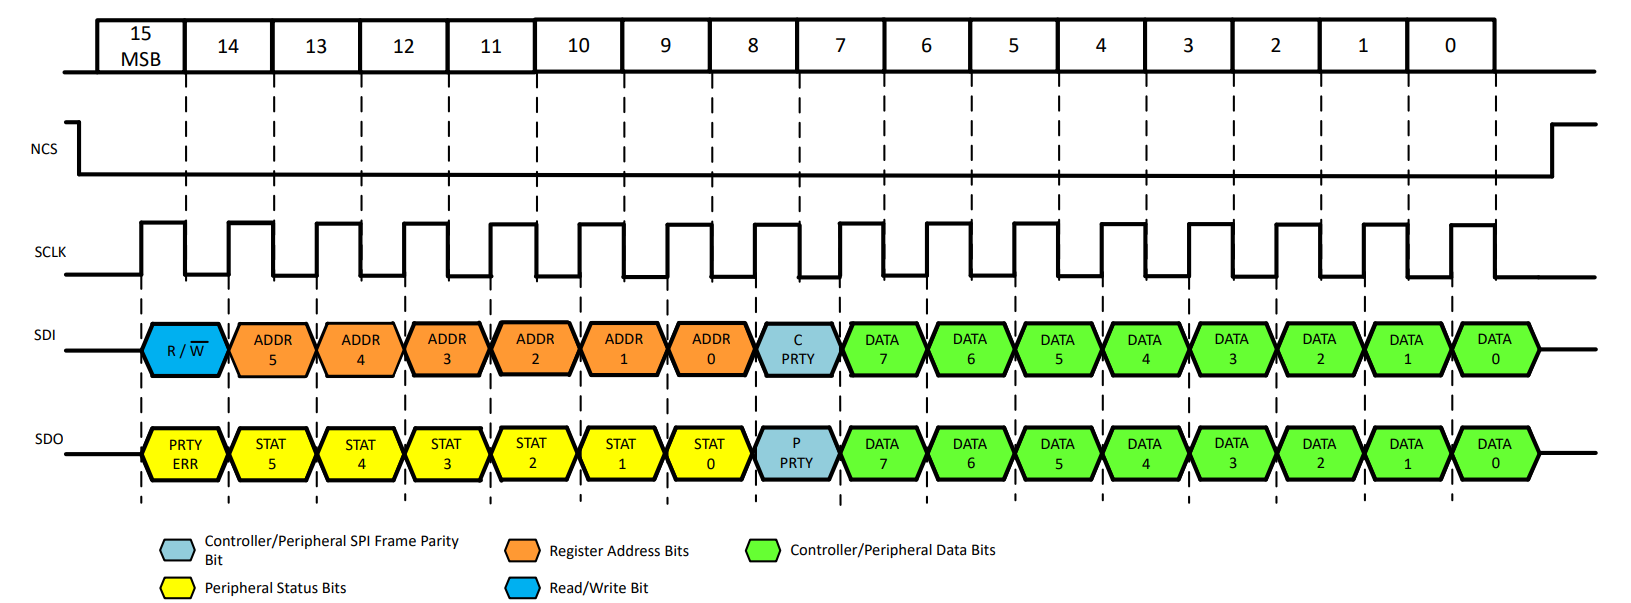
\includegraphics[width=10cm]{figure/SPI Frame.png}
        \caption{SPI数据结构图1}
        \label{SPI数据结构图1}
    \end{figure}
    MCU通过SDI引脚向驱动芯片发送配置数据,通过SDO引脚接收驱动芯片返回的数据。SDI发送数据的第15位为读写选择位,当其选择为write模式或者read模式时,数据收发数据的结构都有所不同,如图\ref{SPI数据结构图2}所示。
    \begin{figure}[ht]
        \centering
        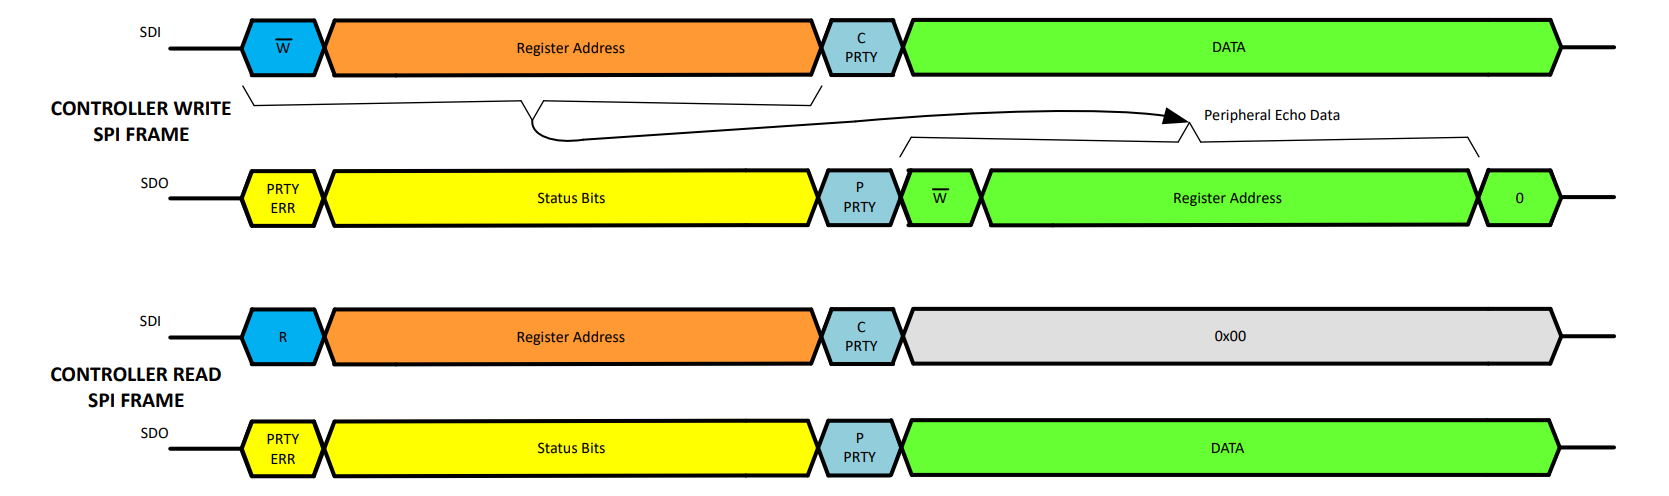
\includegraphics[width=12cm]{figure/SPI Transfer Sequence.png}
        \caption{SPI数据结构图2}
        \label{SPI数据结构图2}
    \end{figure}
    在write模式下,SDI14位-9位为寄存器地址,第8位为奇校验位,7位-0位为寄存器配置数据。SDO第一位为奇校验错误位,用于记录发送数据的奇校验是否通过,未通过校验时该位置1,14位-9位为驱动芯片的状态位,用于反映芯片当前的状态模式,如表\ref{芯片状态表}所示。第8位为奇校验位,7位-0位为写入寄存器的地址。\par
    
     \begin{table}[ht]
        \centering
        \caption{芯片状态表}
        \begin{GDUTtable}{\textwidth}{Y Y}

            \textbf{STATUS BIT }& \textbf{DESCRIPTION}      \\ 
            \hline
            STAT 5 - VDRV\_READY    &   VDRV引脚达到配置电压值时置1  \\ 
            STAT 4 - PULSE\_NUM\_FLT &  发生脉冲数目错误是置1  \\
            STAT 3 - DRV\_PULSE\_FLT &  脉冲发生无响应时置1 \\
            STAT 2 - EE\_CRC\_FLT & 加载内部EEPROM存储器出现CRC错误时置1\\
            STAT <1:0> - DEV\_STATE  &  \makecell{芯片模式:\\
                                        00 - 检测模式\\
                                        01 - 脉冲发生模式\\
                                        10 - 待机模式\\
                                        11 - 睡眠模式} \\

            
      
            \end{GDUTtable}
        \label{芯片状态表}    
         \end{table}
    在read模式下,SDI的14位-9位为读取寄存器地址,7位-0位为0,SDO的7位-0位为该寄存器内存储的数据。
    
    


    
    \paragraph{寄存器配置}
    TUSS4470超声驱动芯片各寄存器的配置如表\ref{寄存器配置}所示。      
    
    \begin{table}[ht]
        \centering
        \caption{寄存器配置}
        
        \begin{GDUTtable}{\textwidth}{Y Y Y Y}
        \textbf{寄存器名} & \textbf{缩写}& \textbf{地址} &\textbf{配置值}\\ 
        \hline
        Bandpass filter settings&BPF\_CONFIG\_1&0x10& 0x25 \\ 
        Bandpass filter settings&BPF\_CONFIG\_2&0x11& 0x00\\ 
        Log-amp configuration&DEV\_CTRL\_1&0x12& 0xB3\\ 
        Log-amp configuration&DEV\_CTRL\_2&0x13& 0x02\\ 
        Log-amp configuration&DEV\_CTRL\_3&0x14& 0x03\\ 
        VDRV Regulator Control&VDRV\_CTRL&0x16& 0x07\\ 
        Echo Interrupt Control &ECHO\_INT\_CONFIG&0x17&0x0F \\   
        Zero Crossing configuration &ZC\_CONFIG&0x18& 0xD4\\  
        Burst pulse configuration &BURST\_PULSE&0x1A& 0x08\\  
        Time of Flight Config&TOF\_CONFIG&0x1B& 0x00\\  
        Fault status bits&DEV\_STAT&0x1C& 0x00\\ 
        Device ID&DEVICE\_ID&0x1D& 0x00\\ 
        Revision ID &REV\_ID&0x1E& 0x00\\ 
        
            \end{GDUTtable}
        \label{寄存器配置}    
         \end{table}
    其中BPF\_CONFIG\_1用于配置带通滤波器的中心频率,该频率需匹配超声波传感器的工作频率,查阅芯片手册可以得知,当寄存器配置为0x25时,带通滤波器的中心频率为301.28$KHz$,与超声波传感器最匹配;\par
    BPF\_CONFIG\_2用于设置滤波器的Q因素,修正滤波器的频率范围;\par
    DEV\_CTRL\_1用于调整对数放大器参数,通过查阅资料,将其设置为0xB3;\par
    DEV\_CTRL\_2用于设置放大器(LNA)的增益;\par
    DEV\_CTRL\_3用于配置脉冲发生的模式,本设计采用IO\_MODE3,故将该寄存器配置为0x03;\par
    VDRV\_CTRL寄存器主要用于配置VDRV引脚的参考电压,当该引脚的实际电压超过参考电压时,驱动芯片的VDRV\_READY状态位置1,然后通过SPI将该状态位返回至MCU芯片。本设计采用12V的驱动电压,根据芯片手册所给出的公式得出该寄存器配置为0x0F;\par
    ECHO\_INT\_CONFIG用于配置VOUT引脚的参考阈值,当VOUT引脚输出电压超过该阈值时,即判断为检测到物体,OUT4拉高。本设计所需的检测距离为$200mm$,根据实验将电压阈值设置为1V,寄存器配置为0x0F;\par
    ZC\_CONFIG寄存器用于配置过零信号,以提高传感器的抗干扰性。选取380mV作为零点,配合OUT4信号进行接近检测,寄存器配置为0xD4;\par
    BURST\_PULSE寄存器的前五位用于配置每个脉冲波的脉冲数,本设计的脉冲数为8,故配置其为0x08;\par
    TOF\_CONFIG寄存器用于待机模式和睡眠模式的设置,本设计只使用到脉冲发生模式和检测模式,暂不需要使用到这两种模式,故配置为0x00;\par
    DEV\_STAT寄存器为芯片的状态寄存器,包括了VDRV状态、脉冲发生状态,可供MCU芯片读取,故不需写入数据,配置为0x00;\par
    DEVICE\_ID和REV\_ID寄存器存放的是芯片的固定参数,无需写入,配置为0x00。
    
    \subsubsection{脉冲发生模块}
    TUSS4470超声驱动芯片有4种脉冲模式来为超声传感器提供激励。在每个模式中,超声发出脉冲的频率取决于外部输入时钟的频率,这可以让使用者产生精确的时钟来匹配超声波传感器的固有频率,从而产生最高的声压水平。在本设计中,将采用脉冲模式1来产生脉冲信号。\par
    在脉冲模式1中,IO2引脚将作为外部时钟输入引脚,IO1作为控制引脚。如图\ref{脉冲模式1}所示,当IO1引脚拉低时,进入脉冲发生模式,在检测到IO2引脚的第一个下降沿时,开始产生脉冲,产生脉冲的数目将通过下降沿的个数来计算。4当产生脉冲的数目达到寄存器内的配置值,或者IO1引脚的信号拉高时,都将退出脉冲发生模式,取决于哪个事件先发生。在进入到脉冲发生模式后,OUTA和OUTB引脚的信号都将取决于IO1和IO2引脚,当需要连续产生多次脉冲时,IO2引脚的信号需要经历低-高-低的过程。
     \begin{figure}[ht]
        \centering
        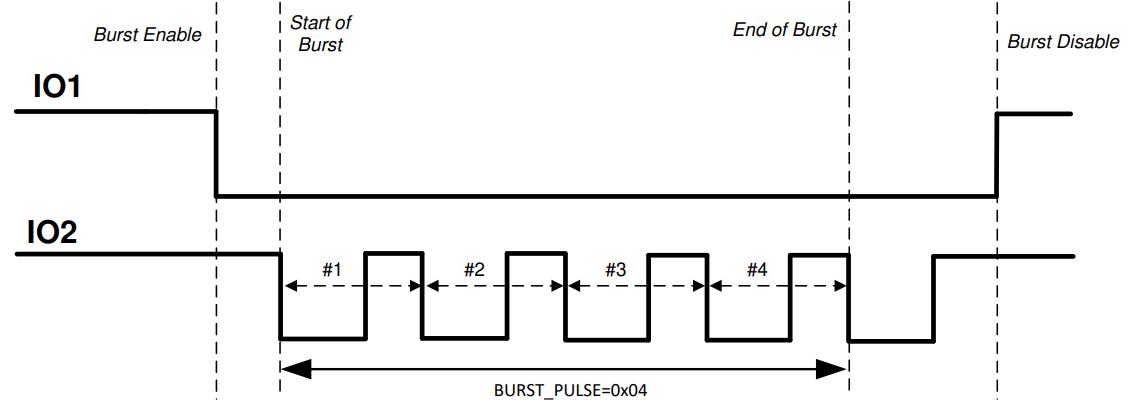
\includegraphics[width=12cm]{figure/IO MODE1.png}
        \caption{脉冲模式1}
        \label{脉冲模式1}
    \end{figure}
    在本设计的脉冲发生模块中,将能产生指定频率,指定脉冲数的脉冲波,如图\ref{单次脉冲程序流程图}为单次脉冲程序流程图,实现的功能为发出一次指定脉冲数、指定频率的脉冲波。
    
        
       \begin{figure}[ht]
        \centering
        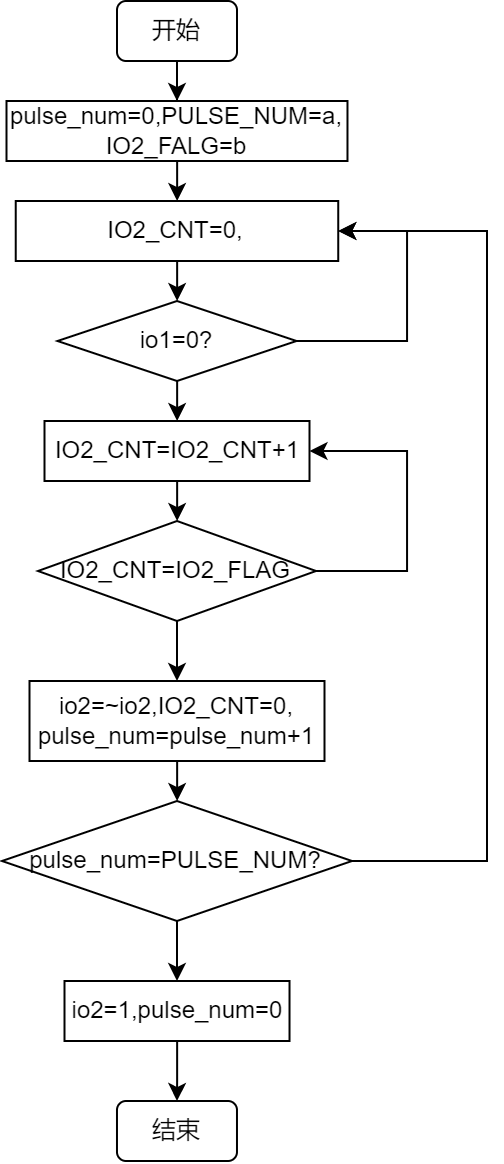
\includegraphics[width=5cm]{figure/single pulse control.png}
        \caption{单次脉冲程序流程图}
        \label{单次脉冲程序流程图}
    \end{figure}

    其中pulse\_num为脉冲数计数位,用于记录当前发射的脉冲数,PULSE\_NUM为预期发射的脉冲数,IO2\_CNT为时钟分频标志位。当io1拉低时,开始产生脉冲,分频标志位开始计数,每当标志位累加到设定值时,io2的状态都会翻转,从而产生特定频率的脉冲信号,其换算公式如式\ref{时钟分频换算},分频后时钟的周期为原时钟周期的2b倍。
    \begin{equation}
        T_2=2bT_1
    \label{时钟分频换算}
    \end{equation}
    当io2翻转次数,即发出的脉冲数等于预期脉冲数时,io2、io1拉高,结束单次脉冲的发送。多次脉冲的发送与检测通过MAIN模块来配合控制,每发射一次脉冲都会进行检测并计数,结束一次检测周期后都会进行状态转移判断。
    
  
    \subsubsection{检测计数模块}
    
    该模块功能在于,对到达指定位置的钢化玻璃进行计数,可以准确得知流水线上到位钢化玻璃的数量,便于后续统计。
    \begin{figure}[ht]
        \centering
        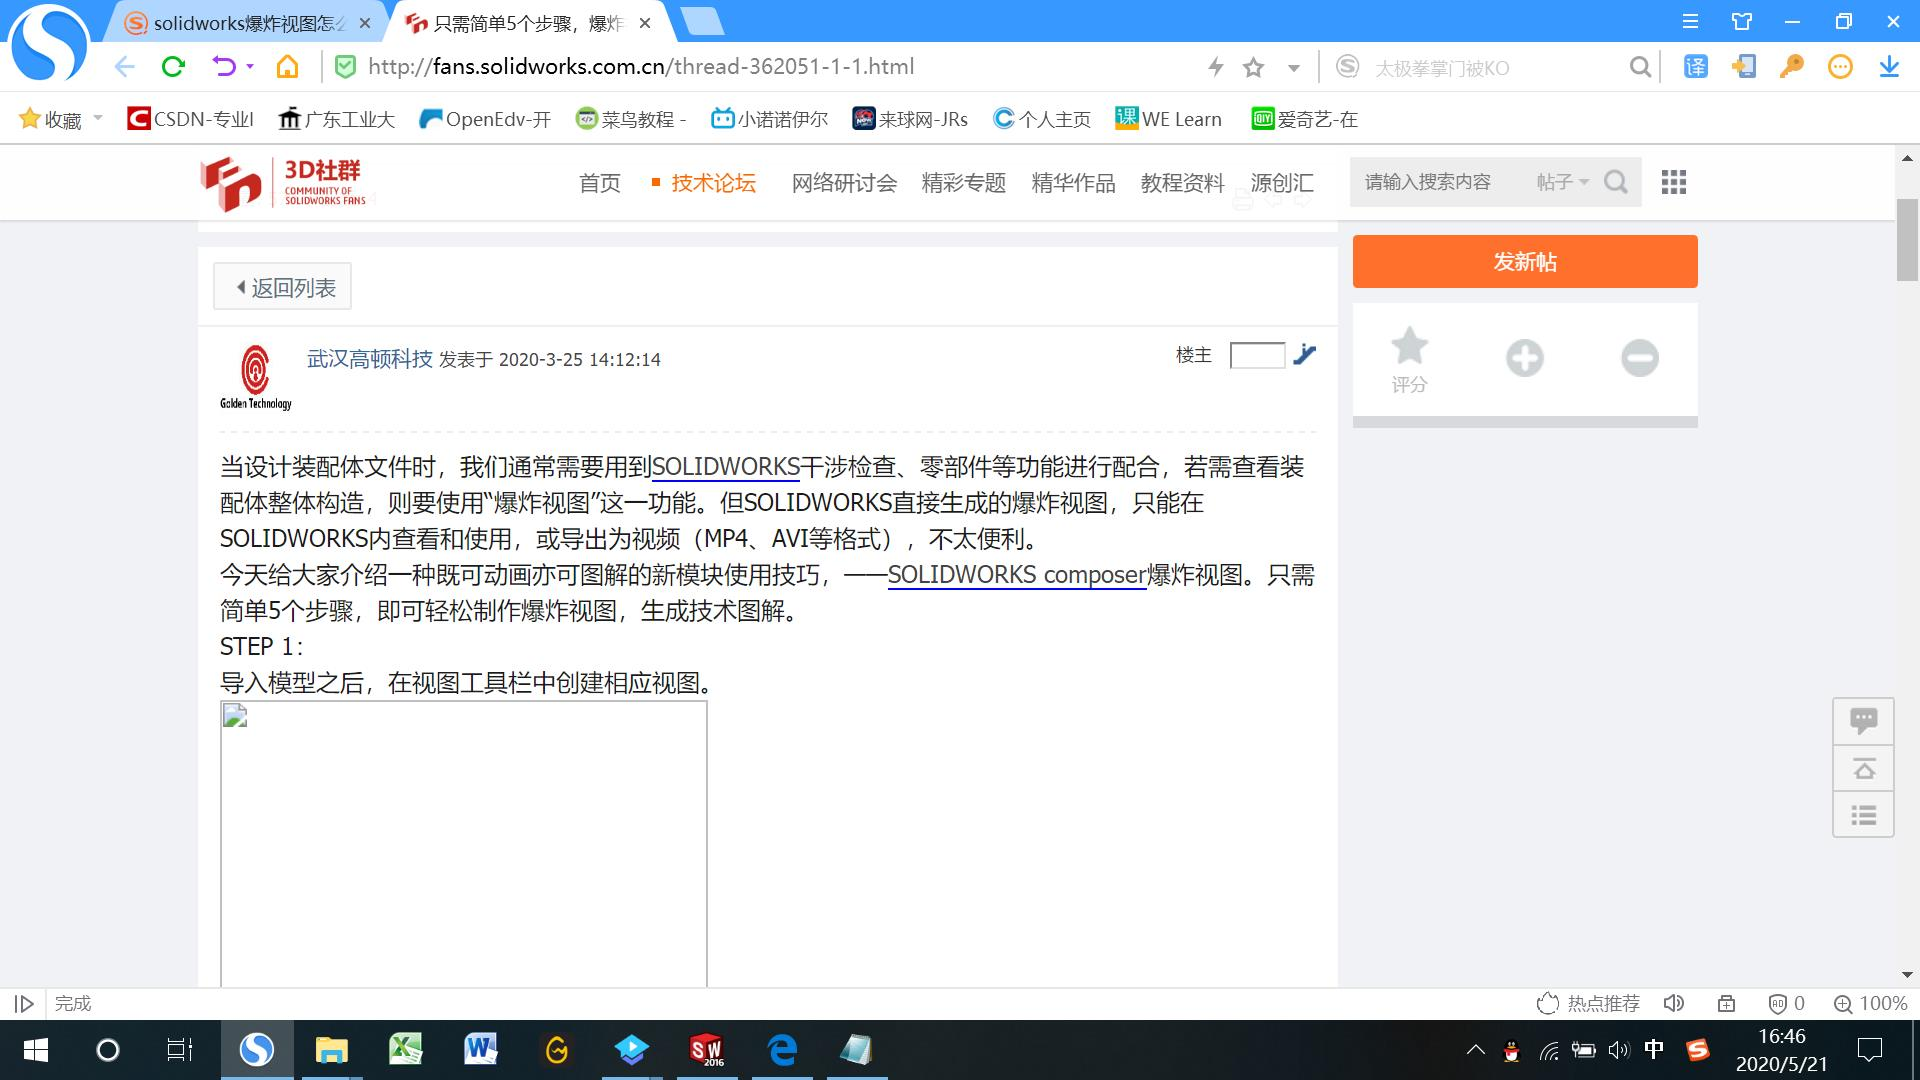
\includegraphics[width=6cm]{figure/1.jpg}
        \caption{检测计数模块程序流程图}
        \label{检测计数模块程序流程图}
    \end{figure}

    其功能实现流程如图\ref{检测计数模块程序流程图}示:当一块玻璃到位后,到位检测指示灯LED1变亮,CPLD芯片从CT\_1口得到一个高电平信号,计数寄存器object\_num加1;当钢化玻璃离开检测区域后,检测指示灯灭,等待下一块玻璃到位。\par
   
    
    \subsubsection{仿真模拟}
    \paragraph{仿真环境的搭建}
    在完成程序设计部分的工作后,就要开始搭建环境,来完成代码的编写,以及时序调试与仿真,来验证其可行性,本设计采取QUARTUS II配合MODELSIM联合仿真的测试方式。\par
    Quartus II是由Intel公司推出的FPGA设计软件。FPGA是一种可编程逻辑器件,Quartus II软件可以用于FPGA设计的各个环节,包括原理图设计、硬件描述语言(HDL)编程、仿真、综合、布局布线等。Quartus II软件支持的HDL包括VHDL和Verilog。使用Quartus II软件可以快速完成FPGA的设计、验证和调试;
    ModelSim是一种常用的数字电路仿真工具,由Mentor Graphics公司开发。它支持VHDL和Verilog两种硬件描述语言,并且支持多种硬件平台,包括Intel FPGA、Altera FPGA等。\par
    本设计中QUARTUS II使用的版本为18.0,MODELSIM采用的版本为10.1,软件运行的环境为64bit-win10系统。\par
    \paragraph{工程文件的创建}
    QUARTUS II在编写代码前需要建立工程文件。首先打开Quartus软件,选择File -> New Project Wizard。
    在弹出的New Project Wizard窗口中,选择Create a new project选项,然后单击Next。
    在下一个窗口中,输入项目名称和存储位置,并选择要使用的FPGA器件系列。然后单击Next。
    在接下来的窗口中,选择要添加到项目中的源文件类型,例如VHDL、Verilog等,并选择项目的顶层实体文件。然后单击Next。
    在下一个窗口中,选择要使用的IP核和约束文件,如果没有,则可以跳过这一步。然后单击Next。
    在接下来的窗口中,选择要使用的EDA工具,例如ModelSim等。然后单击Next。
    在最后一个窗口中,查看项目设置的摘要,并单击Finish以创建工程。
    完成这些步骤后,Quartus将创建一个新的工程文件夹,其中包含工程文件源文件和约束文件。在文件夹中可以新建顶层模块和各子模块的源文件,顶层模块的模块名必须要和工程名保持一致。在本设计中,顶层模块不实现任何逻辑,只起到端口例化,连接各个子模块的作用。\par
    在进行仿真模拟之前,需要选择仿真工具,创建TESTBENCH文件。在Tool->Options->EDA Tool Options中,将 Modelsim 的地址改为 Modelsim 启动程序的路径;在Assignments -> Simulation中选择Tool name为ModelSim;然后选择Processing->start->Start TESTBENCH Template Writer,如果设置正确,会在工程路径 simulation/modelsim 下产生 .vt 文件,TESTBENCH就将在这个文件中进行编写。在完成上述设置后,还需要将 TESTBENCH 添加到工程中,点击Assignments -> Settings -> Simulation,
    在 Compile test bench 选项中,选择 new,设置 Test bench name,并通过 File name 查找的方式,将上一步生成的 .vt 文件添加到工程中。重新一键编译后,点击Tools->Run simulation Tool->RTL Simulation进行仿真。
    
    \paragraph{仿真激励文件编写}
    在QUARTUS II软件中,需要编写TESTBENCH文件来为程序提供虚拟的外部激励以进行仿真调试,在本设计中,程序包含的外部激励端口有gclk、rstn、out3、out4、ct1。如图\ref{TESTBENCH结构图}所示,TESTBENCH的结构中包括了信号声明、复位信号产生、时钟生成、外部激励生成、模块例化、自校验、停止仿真。\par
    \begin{figure}[ht]
        \centering
        \includegraphics[width=10cm]{figure/TESTBENCH structure.png}
        \caption{TESTBENCH结构图}
        \label{TESTBENCH结构图}
    \end{figure}
    如公式\ref{周期计算公式}所示,当选取时钟的频率为27$MHz$时,时钟周期为$\frac{1}{27}\mu s$,在仿真激励中则需要每过$\frac{1}{54}
   \mu s$将gclk信号反转一次。
    \begin{equation}
        T=\frac{2\pi}{f}
        \label{周期计算公式}
    \end{equation}
    对于其它的激励信号,在程序开始时,复位信号拉低,程序复位,延时一段时间后,复位信号拉高,程序开始运行。out3和out4信号一直保持着拉高状态。
	
	\newpage
    \paragraph{波形仿真}
    在完成上述配置后,编译程序,就可以在MODELSIM软件内进行仿真,调试波形。
    
    
      \begin{figure}[ht]
      	\centering
  		\subfloat[超声波接近传感器整体仿真波形图]{
  		\begin{minipage}[b]{0.7\textwidth}
  			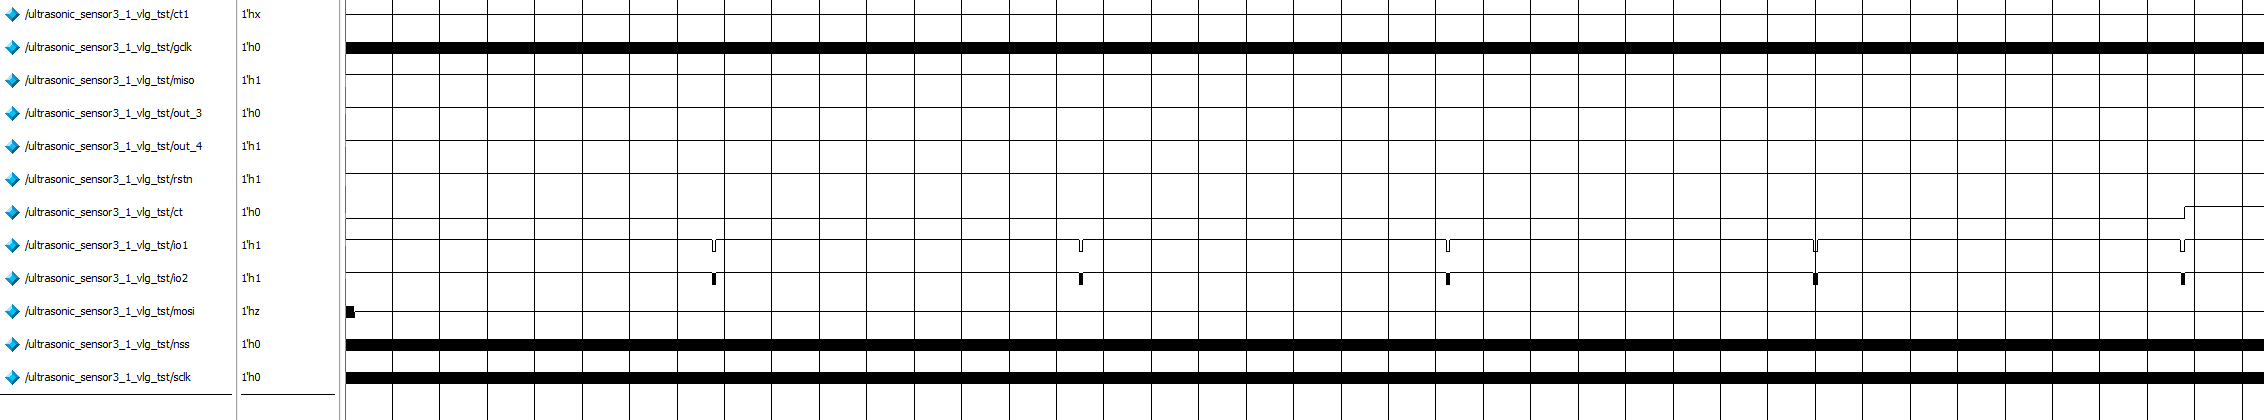
\includegraphics[width=12cm]{figure/overall wave simulation.png}
  		\end{minipage}
  		\label{超声波接近传感器整体仿真波形图}
  	}\\
	\centering
	\subfloat[SPI通信仿真波形图]{
		\begin{minipage}[b]{0.7\textwidth}
			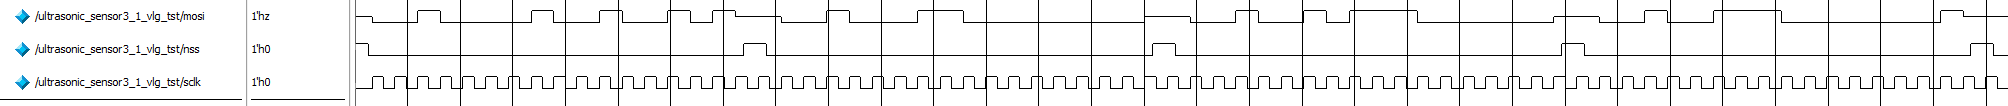
\includegraphics[width=12cm]{figure/spi wave simulation.png}
		\end{minipage}
		\label{SPI通信仿真波形图}
	}\\
	\subfloat[脉冲信号产生仿真波形图]{
		\begin{minipage}[b]{0.7\textwidth}
			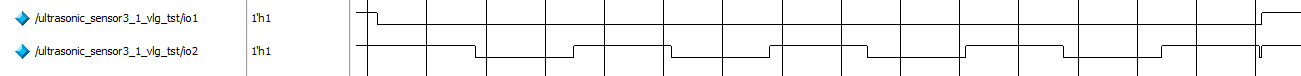
\includegraphics[width=12cm]{figure/pulse wave simulation.png}
		\end{minipage}
		\label{脉冲信号产生仿真波形图}
	}

	\caption{超声波接近传感器程序仿真波形图}
	\label{超声波接近传感器程序仿真波形图}
\end{figure}


    如图\ref{超声波接近传感器整体仿真波形图}所示,可以在MODELSIM软件中看到各个端口整体输出的波形状态。图\ref{SPI通信仿真波形图}为SPI通信部分的仿真波形,MOSI引脚可以正常向TUSS4470芯片发送配置数据,在发送完成数据后,如图\ref{脉冲信号产生仿真波形图},io1和io2端口配合产生脉冲波。在产生完成指定的脉冲数后,检测到外部激励OUT4信号拉高,程序判断为检测到物体,CT拉高,检测指示LED灯亮。\par
    \subsection{本章小结}
    本章首先介绍了超声波接近传感器的检测原理和检测策略,采用多次发射脉冲波,检测是否达到次数阈值的检测策略。然后讲解了程序的总体设计框图,将程序分为了主控制模块、SPI通信模块、脉冲信号产生模块,分别详细介绍了各个模块的基本功能、实现原理、程序算法。最后讲解了进行仿真模拟所进行的流程,包括仿真环境搭建、工程文件的创建、仿真激励文件的编写以及最后使用MODELSIM软件进行波形仿真。下一章将介绍实物制作以及实验设计部分的工作。
    